\chapter{Signal Simulation}
Because the signal process for \dbrem occurs between outgoing particles from the collision and nuclei within the detector, it must be built into the \gf simulation of the detector reponse instead of directly imported as an initial state from an event generator. A custom process was created to accomplish this \cite{Eichlersmith_2023}, and the techniques used therein are described in this chapter. The cross section and kinematics produced by the process are compared to an existing \mg package \cite{madgraph_2014, darkgauge} which provides an accurate implementation of the underlying matrix element based on an input field theory model.
The initial state used for signal simulation is the DY process decaying to two muons, with identical settings to the background DY generation other than the enabled signal process. 

In order to efficiently produce signal events, $\epsilon$ is set to one and the cross section is multiplied by fixed biasing factors for each \aprime mass. 
Additionally, the interaction is only enabled within the HCAL endcap and is disabled after the \aprime is produced to avoid non-physical events with multiple \dbrem interactions that could be caused by the increased interaction probability.
The increased interaction rate biases events towards the center of the detector, as deeper regions see a reduced number of muons due to earlier \dbrem interactions.
This bias is rougly proportional to the fraction of muons undergoing \dbrem squared, so the bias factors are selected to have rates less than 5$\%$. 
A table of the biasing factors used, as well as the corresponding signal rate per incident muon, is presented in \cref{table:dbrem_biasfactors}.
Simulated events that have no \dbrem or do not pass the base event selection are discarded.

\begin{table}[h]
    \centering
    \spacerows{1.2}
    \begin{center}
        \begin{tabular}{@{}l rr@{}}
            \toprule
            \aprime Mass (\SI{}{\giga\eV})& Bias Factor & Interaction Rate\\
            \midrule
            0.2&800&0.22\\
            0.4&1200&0.10\\
            0.6&1600&0.06\\
            0.8&2500&0.04\\
            1.0&3200&0.04\\
            \bottomrule
        \end{tabular}
        \caption{
            Bias factors used in \dbrem generation.
        }
        \label{table:dbrem_biasfactors}
    \end{center}
\end{table}

\section{\ww}
\label{sec:wwApprox}
In order to simplify the kinematics of the 2 particle to 3 particle process of \dbrem, where the initial incoming lepton interacts with a nucleus to add an \aprime to the final state, an method known as the \ww approximation \cite{vonWeizsacker:1934nji,Williams:1935dka} is frequently used in fixed-target searches where the interaction must be simulated with the response of a detector \cite{Bjorken_2009,Andreas_2012}.
The \ww approximation is a semiclassical approximation, in which the nearly transverse electromagnetic field generated by a fast moving charged particle is approximated by a real photon. 
Thus, the interaction is approximated as a charged particle interacting with a photon field to produce a \aprime, ignoring the interaction with the nucleus and reducing the calculation to a 2 particle to 2 particle process with much simpler kinematic integrals.

As a further simplification, the necessary phase space for the interaction can be reduced by assuming that the outgoing \aprime and lepton are nearly collinear and that the majority of the outgoing kinetic energy is carried by the massive \aprime.
For the approximation to hold, the energy of the beam must be much larger than the mass of the new particle (in this case, the \aprime) and the lepton mass so that the assumption of only transverse interactions with the photon fields holds. 

For a high energy muon incident on some nucleus in the detector, the calculation begins by finding the effective photon flux integrated over t, the four-momentum transfer in the collision. 
This integrated flux, $\chi$, is shown in \Cref{eq:chi}, where $E_0$ is the initial muon energy, $m_\mu$ is the muon mass, $m_A$ is the dark photon mass, $m_p$ is the proton mass, $\mu_p$ is the magnetic moment of the proton, and Z and A are the proton number and atomic mass of the target material.
The first term in this integral represents the  elastic scattering component, proportional to the electron screening form factor $a$ and finite nuclear size $d$, which dominates at small \aprime masses .
The second term represents inelastic scatters, proportional to the inelastic atomic form factor $a'$, which itself is split into nuclear and atomic form factors and becomes comparable to the elastic term for larger \aprime masses ($m_A'>$\SI{1}{\giga\eV}).
More information on this calculation can be found in references \cite{kim_1973} and \cite{tsai_1974}. 

\begin{equation}
	\label{eq:chi}
	\chi = \int^{E_0^2}_{t_{min}} dt \left( \frac{Z^2a^4t^2}{(1+a^2t)^2(1+t/d)^2}+\frac{Za_p^4t^2}{(1+a_p^2t)^2(1+t/0.71)^8}\left(1+\frac{t(\mu_p^2-1)}{4m_p^2}\right)^2\right)\frac{t-t_{min}}{t^2}
\end{equation}

\begin{equation}
	\label{eq:utilde}
	\tilde{u} = -xE_0^2\theta^2 - m_A^2\frac{1-x}{x} - m_\mu^2x
	\quad
	t_{min} = \left(\frac{\tilde{u}}{2E_0(1-x)}\right)^2
\end{equation}

\begin{equation}
	\label{eq:adefs}
	a = \frac{111.0}{m_e Z^{1/3}}
	\quad
	a_p = \frac{773.0}{m_e Z^{2/3}}
	\quad
	d = \frac{0.164}{A^{2/3}}
\end{equation}

Given this effective photon flux, the total cross section from the \ww approximation is shown in \Cref{eq:fullCX} \cite{Bjorken_2009}, where $\sigma$ is the total cross section and $\alpha_{EW}$ is the fine structure constant (1/137).
To reduce computation time the outgoing dark photon angle, $\theta$, is limited to 0.3 and terms of order $m_\mu^2$ in the initial matrix element are dropped.
As the vast majority of dark photons produced have very small scattering angles and the muon mass is small with respect to the other terms in the matrix element, these approximations have negligible impacts on the total cross section calculation.

\begin{equation}
	\label{eq:fullCX}
        \sigma = \frac{pb}{GeV} \int_0^{0.3} \int_0^{\min(1-m_\mu/E_0,1-m_A/E_0)} 2 \alpha_{EW}^3\epsilon^2 \sqrt{x^2E_0^2 - m_A^2}E_0(1-x) 
	    \frac{\chi(x,\theta)}{\tilde{u}^2} \mathcal{A}^2
~dx~d\theta
\end{equation}
\begin{equation}
	\label{eq:afunc}
	\mathcal{A}^2 = 2\frac{2-2x+x^2}{1-x}+\frac{4(m_A^2+2m_\mu^2)}{\tilde{u}^2}(\tilde{u}x + m_A^2(1-x) + m_\mu^2x^2)
\end{equation}

While this method of calculating the cross section forms a good approximation of the total rate of \dbrem interactions, it does not effectively simulate the outgoing kinematics for the scattered lepton, which are of particular interest in this analysis as the outgoing muon will be the only final state particle that is visible in the detector.
Because the interaction is approximated as a scattering of the incident lepton with a photon field, any scattering of the nucleus itself is not included in this method.
The produced dark photon is kinematically favored to carry most of the outgoing energy, so corrections due to the missing nucleus are largely negligible.
For the scattered electron, the outgoing energy tends to be very small, and is often comparible to the energy of the nucleus.

As a demonstration, the distribution of the outgoing muon energy created using the differential \ww approximation is compared to simulations using \mg in \Cref{fig:wwMgComp}. 
The most dramatic differences are at very large muon energies, where the \ww approximation predicts greatly increased rates for muons to retain nearly all of the incident kinetic energy.
As muons in this region are rare and this search is not sensitive to muons which retain most of the incident energy, this disagreement in large muon energies is negligible.
The disagreement at very small energies (x$<0.02$) is of much greater concern. 
These very low energy muons can have very different signatures in the detector with slight changes in momentum, as a difference of a few \SI{}{\giga\eV} can greatly alter the probability of the muon to reach the muon chambers before being fully absorbed or deflected away by the magnetic field.

\begin{figure}[h]
	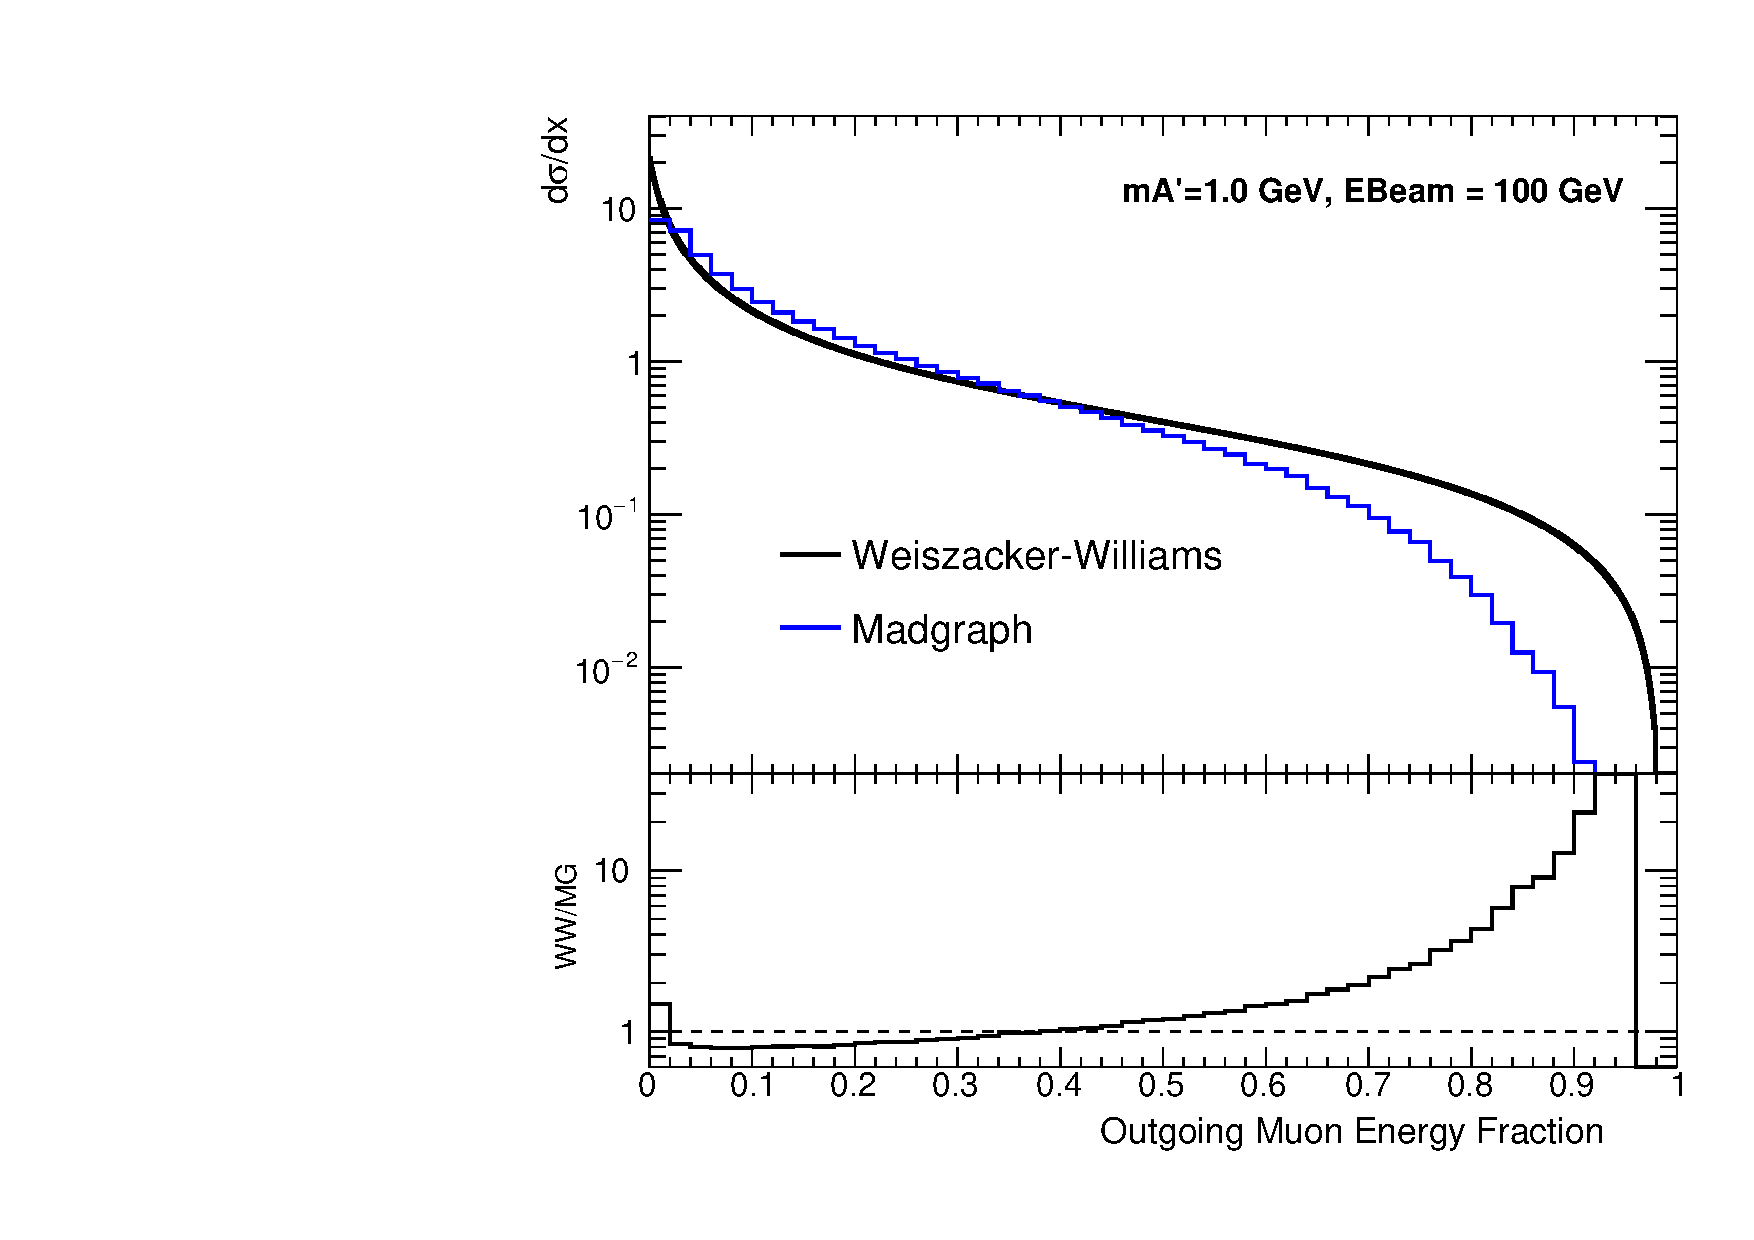
\includegraphics[width=0.9\textwidth]{figures/wwXcomp.pdf}
	\caption[\ww and \mg Outgoing Energy]{The fraction of the initial kinetic energy carried by the outgoing muon in \mg and using the \ww approximation. While the differences at large energy fractions are a small fraction of events and do not match the target kinematics of this search, the sharp peak seen at very low energies using \ww could result in substantial inaccuracy in predictions of the signal efficiency.}
	\label{fig:wwMgComp}
\end{figure}

While the total cross section from \ww sees good agreement with \mg and can be used to determine the probability of interaction, because of the potential sensitivity of the signal efficiency to small changes in low energy muon kinematics and the significant inaccuracy seen when predicting them using the \ww approximation, an alternate method of simulating the outgoing muon kinematics is required.

\section{Technique}
\label{sec:technique}

The physics of \dbrem was implemented in \gf via the creation of an additional physics process class describing the interaction. 
\gf discretizes the simulation of physics into "steps" of time. 
During each step of particle simulation, \gf uses the total cross section all possible physics interactions for that particle to determine which, if any, interactions should occur, then modifies the particle kinematics and generates secondaries as necessary. 
The total cross section is calculated by performing a numerical integration of the \ww approximation.
The relative accuracy of this approximation for the energy range used in CMS is shown in \cref{fig:mu_xsec}.
The result depends on the mass of the \aprime,  the energy of the incident muon, and the material it passes through. 

To circumvent the inaccuracies from the missing nucleus in \ww, the simulation does not construct outgoing muons by sampling from the differential \ww cross section and instead a technique of scaling existing \mg events to the desired incident muon energy was developed. 

\begin{figure}[!htbp]
    \centering
    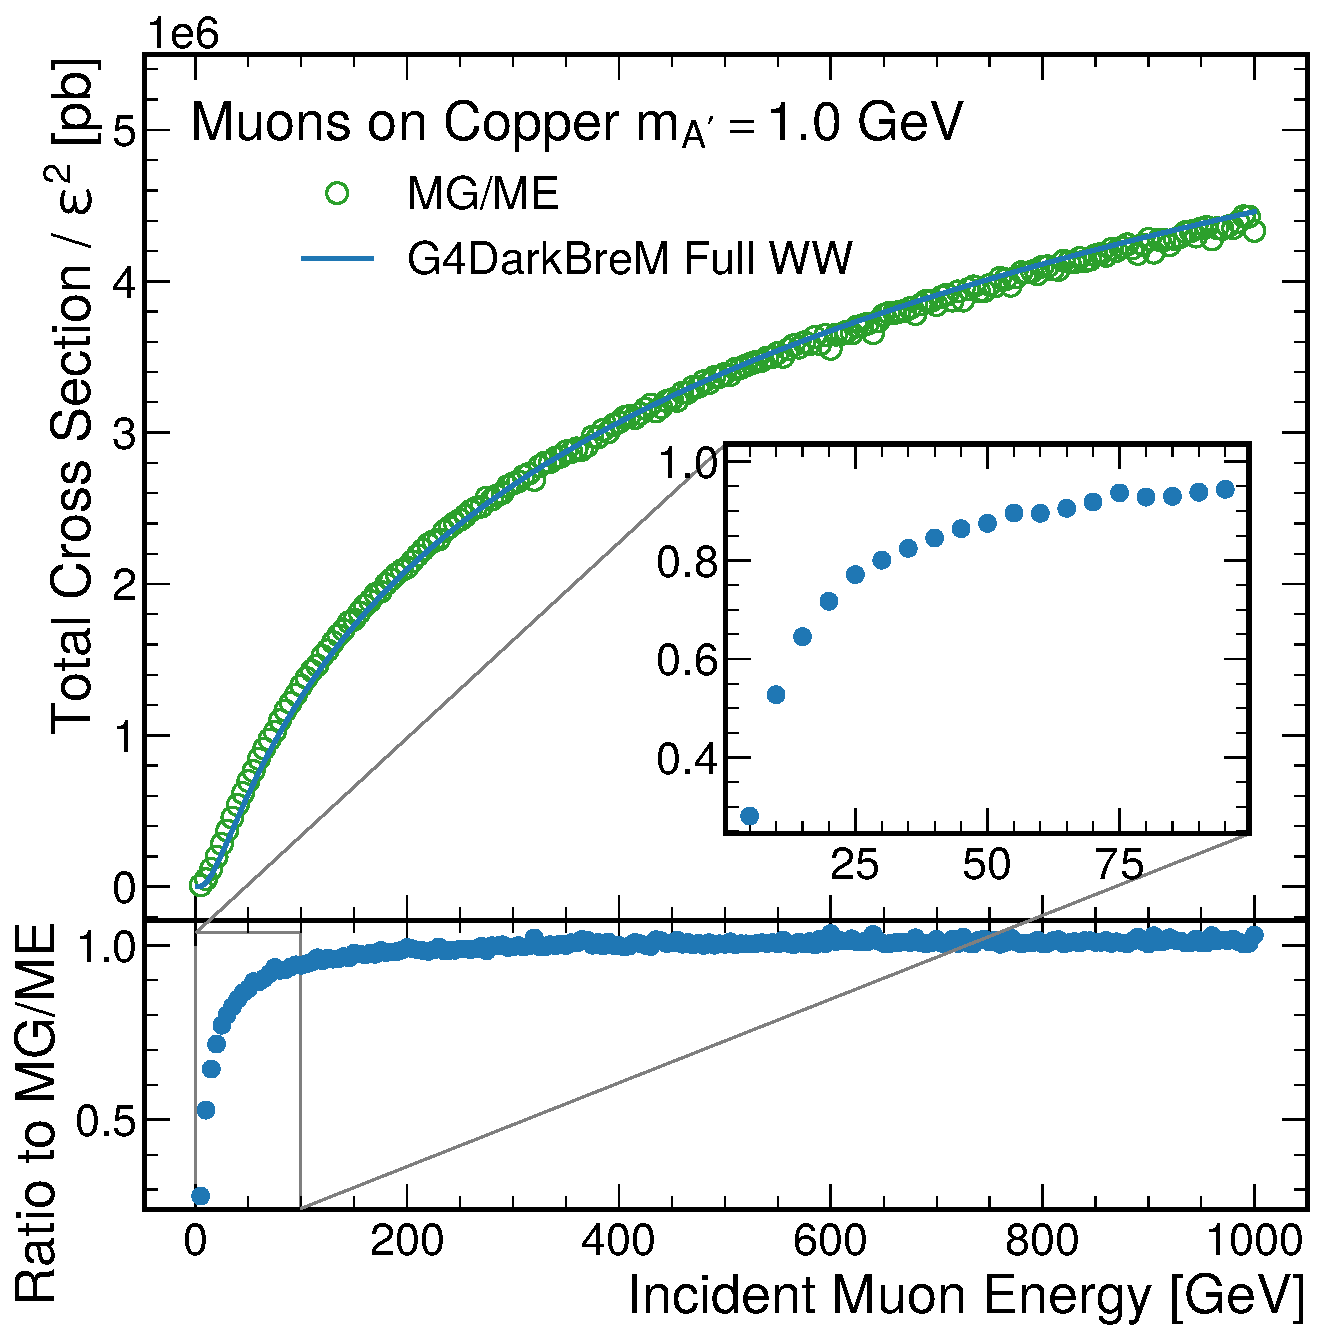
\includegraphics[width=\textwidth]{figures/mu_xsec.pdf}
    \caption[
        The \dbrem cross section.
    ]{
        The total \dbrem cross section for muons incident on copper. 
    }
    \label{fig:mu_xsec}
\end{figure}

Through study of \mg events produced over a range of incident muon energies, two variables with distributions that vary slowly with incident energy were identified: the fraction of the incident kinetic energy imparted to the scattered muon and the transverse momentum of that muon with respect to the incident particle (\cref{fig:efrac_pt}). 
Because of this slow variation with incident energy, these variables can be sampled from a set of previously simulated \mg events at a ``nearby'' energy and rescaled to the desired initial energy without introducing large error. 
The two variables are correlated, so they must be sampled together. 
The scaling from a sampled \mg incident energy to the actual \gf incident energy has been found effective over a wide range; nevertheless, the differences become more pronounced as the relative distance between the sampled and true incident energies increases.
The impact of these variations is limited by using fine-binned energies in the sampled \mg libraries, and a systematic uncertainty is assessed by scaling each event to the second-nearest available energy to estimate the maximum impact that could be produced from the chosen binning. 

\begin{figure}[!htbp]
    \centering
    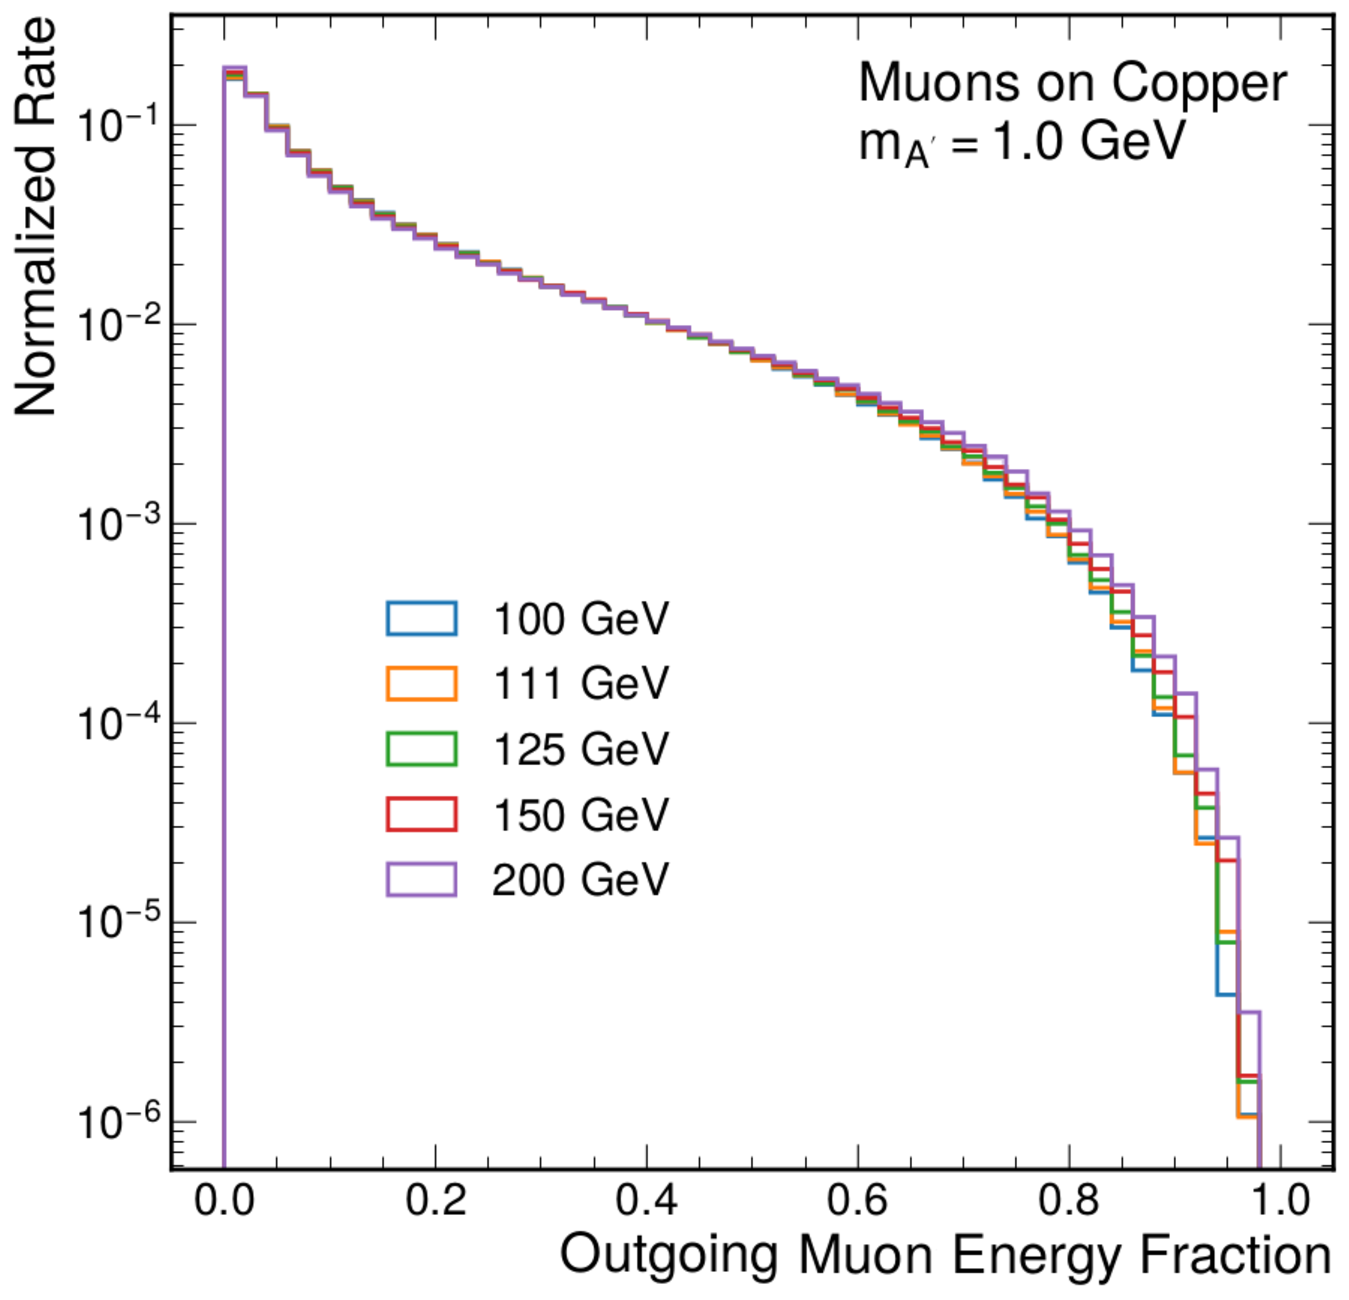
\includegraphics[width=0.45\textwidth]{figures/muon_energy_comp_efrac.pdf}
    \hspace{0.01\textwidth}
    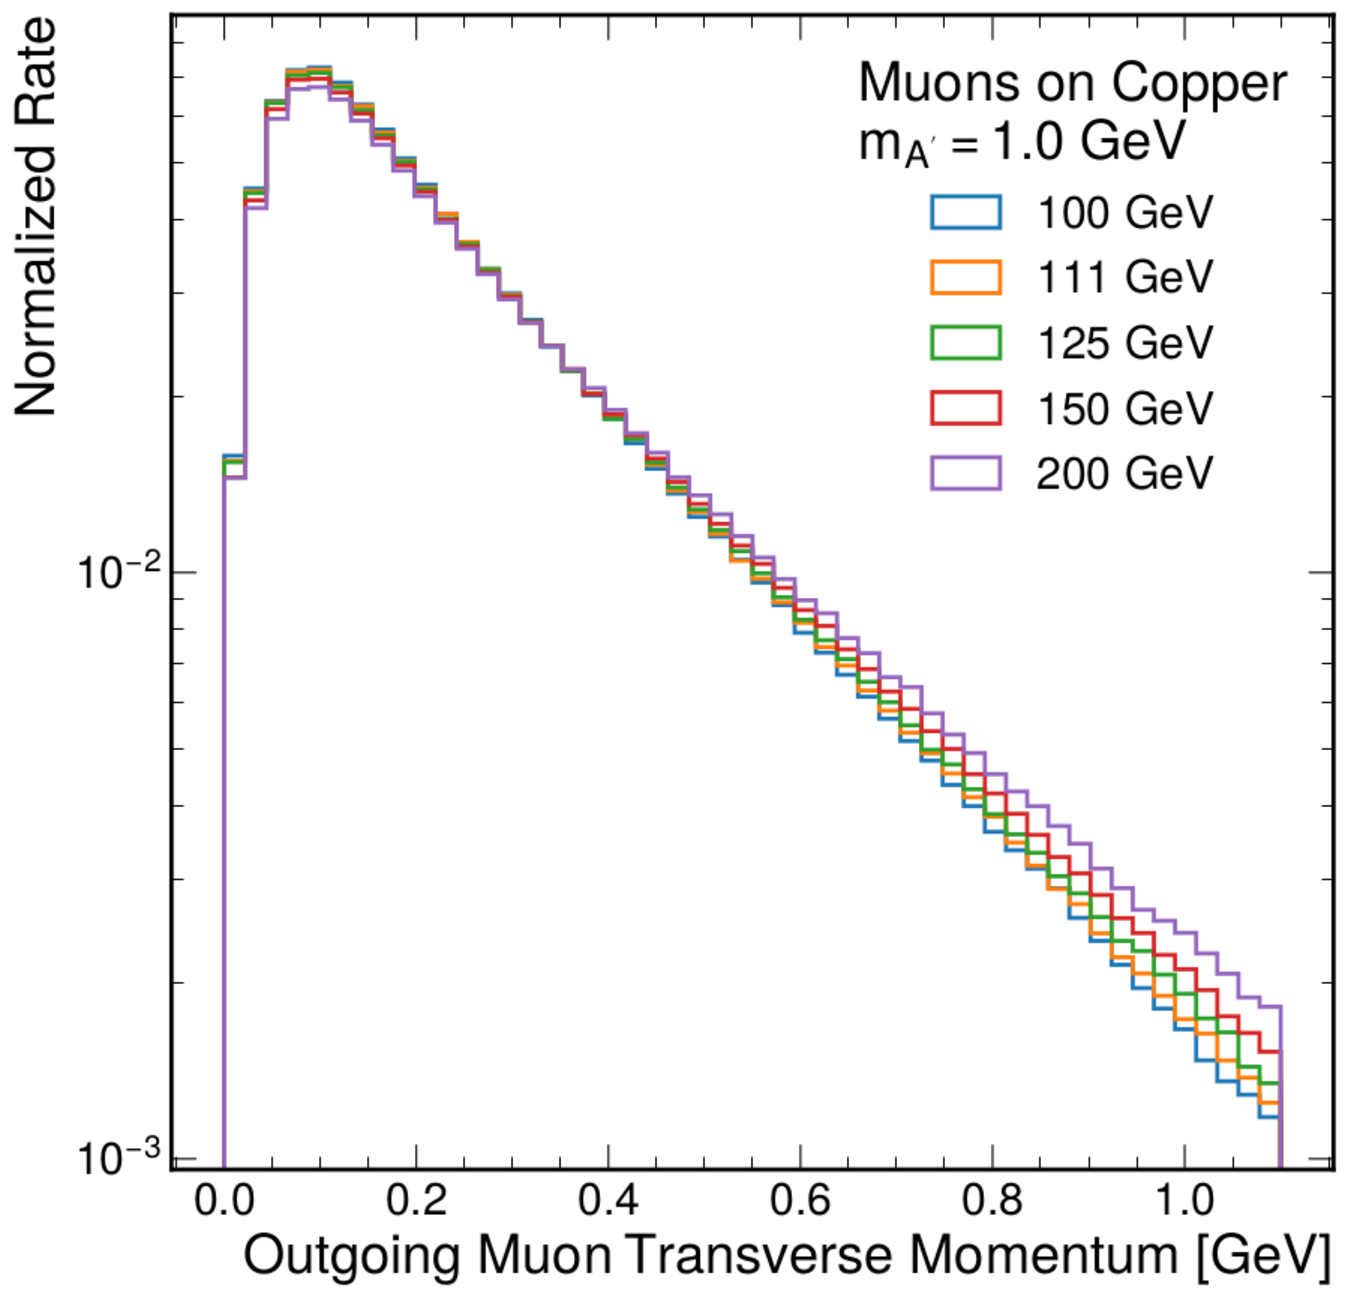
\includegraphics[width=0.45\textwidth]{figures/muon_energy_comp_pt.pdf}
    \caption[
        Sampling variables used for \dbrem simulation.
    ]{
        The outgoing muon energy fraction (left) and transverse (right) for muons incident on copper. Despite large shifts in the incident muon energy, the two distributions of the two variables remain relatively constant. 
    }
    \label{fig:efrac_pt}
\end{figure}

When \gf determines that a \dbrem event should occur in the simulation, the process selects a random event from the nearest available muon energy and target material in the loaded \mg library. 
\gf then creates a muon with the same transverse momentum as the sampled event and scales the outgoing kinetic energy to match the fraction of incident kinetic energy of the sampled muon, then randomly selects an azimuthal angle with respect to the initial muon momentum. 
In the rare case where the rescaled total energy of the deflected muon would be smaller than the selected transverse momentum, alternate events are sampled until one is found with final energy larger than its transverse momentum. 

The simulation assumes that the scattered nucleus does not receive sufficient momentum to produce an observable signal in the detector; therefore, no \gf particle for the scattered nucleus is created and, as a result, energy and momentum cannot be precisely conserved using only the \aprime and scattered muon. 
In searches with visible \aprime and muon signatures this effect would introduce un-accounted for correlations between the secondaries, but with an invisible \aprime only the muon requires correct kinematics and an arbitrary outgoing \aprime can be produced.  
The simulation produces an \aprime using only conservation of momentum so that the incident muon can be reconstructed from simulation-level information about the \aprime and the scattered muon.
No physics processes are been implemented for the emitted \aprime to ensure that it remains invisible to the detector.

The kinematics of the outgoing muon depend weakly on the composition of the target material.
The core assumptions of the scaling technique, slow variation of transverse momentum and outgoing energy fraction spectra with respect to incident energy, are found to remain valid across a wide range of target materials while the underlying distributions of those variables have small dependences on the material type (\cref{fig:dbrem_material}).
Because the kinematics have small variation with scattering material, all \dbrem interactions in this analysis are scaled from samples produced with a copper target, which is the most frequent \dbrem initiating material in the CMS HCAL endcap (See Table \ref{table:dbrem_material}).

Lastly, the process is only enabled within the HCAL endcap and, separately, the ECAL endcap (\Cref{fig:HEbrems,fig:EEbrems}).
Only those regions are considered for potential signal sources due to the large uncertainty or low total material in other regions of the detector and surrounding support structure.

\begin{figure}[h]
	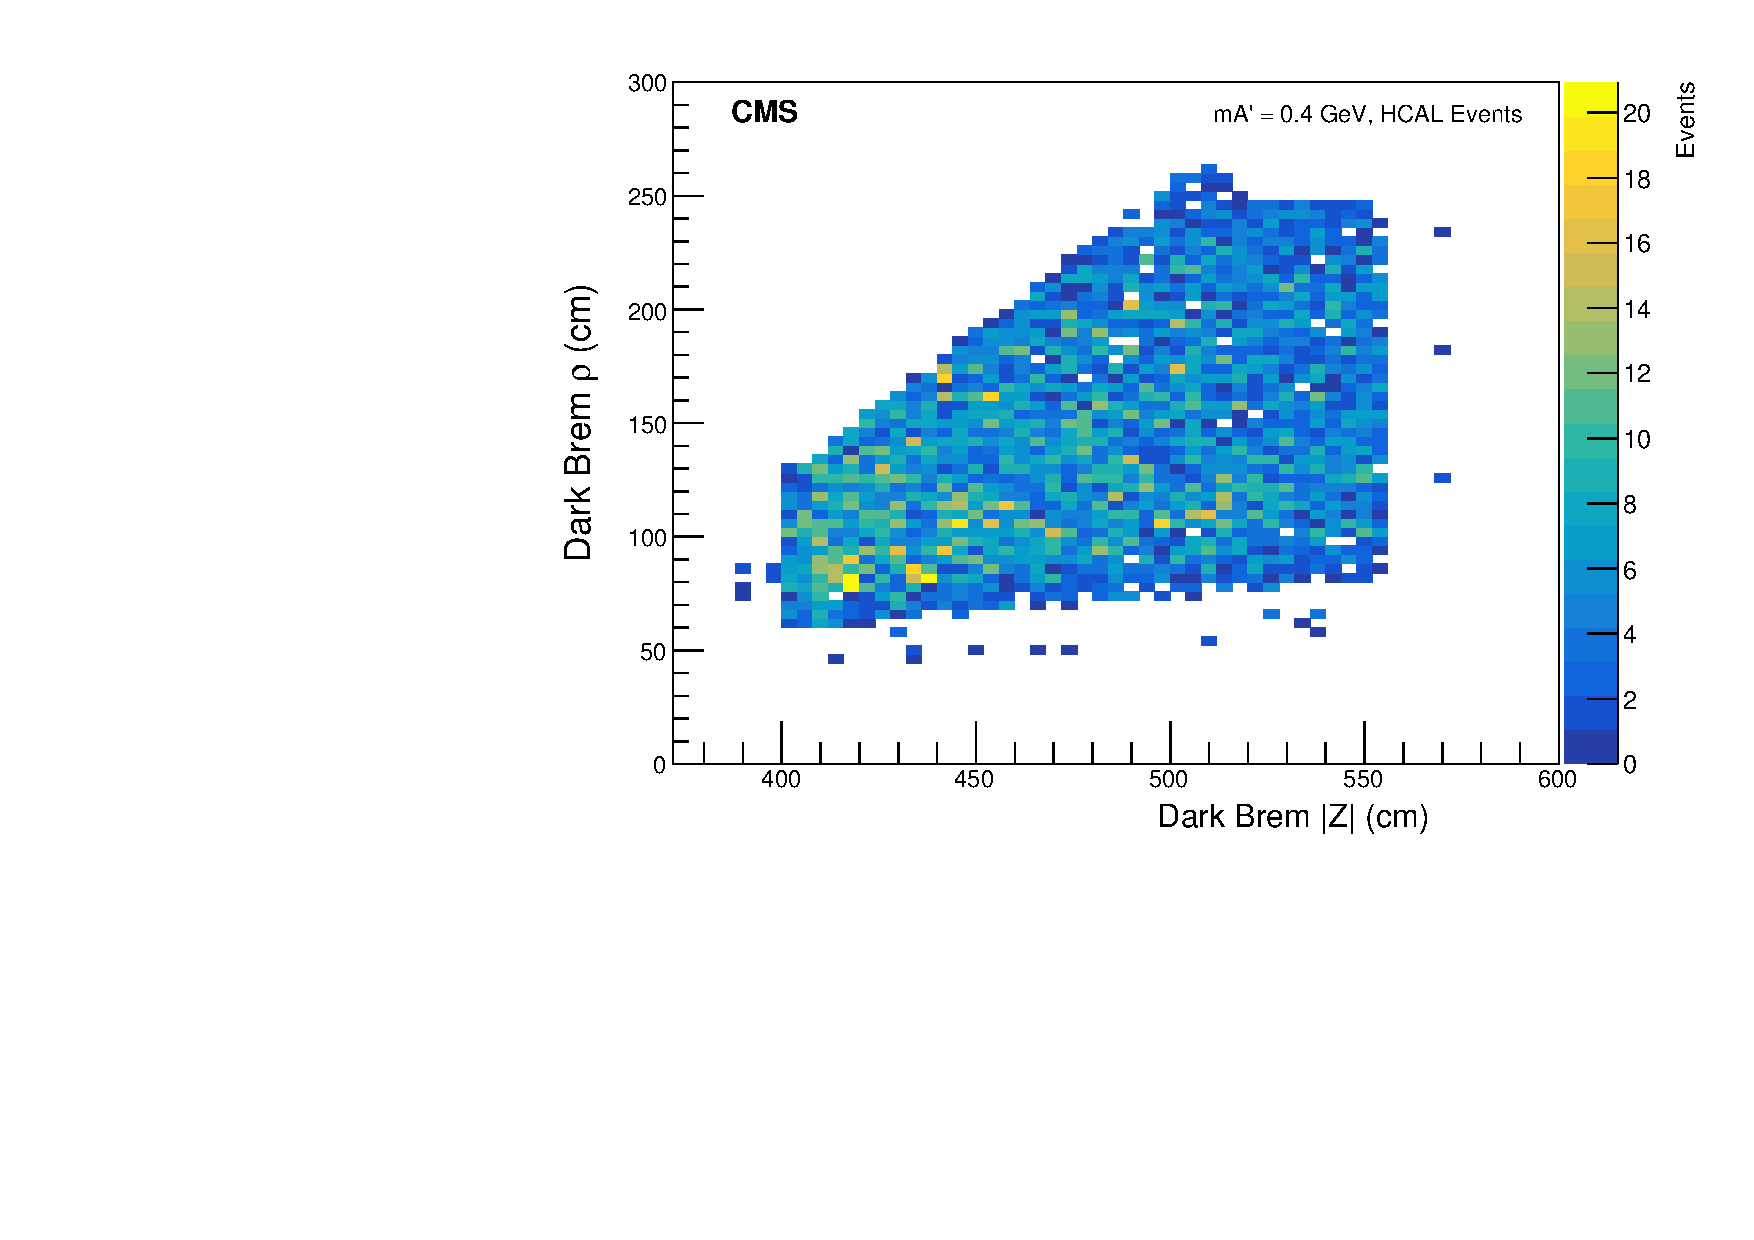
\includegraphics[width=0.9\textwidth]{figures/HCALbrems.pdf}
	\centering
	\caption{The locations of simulated \dbrem events within the CMS HCAL endcap}
	\label{fig:HEbrems}
\end{figure}

\begin{figure}[h]
	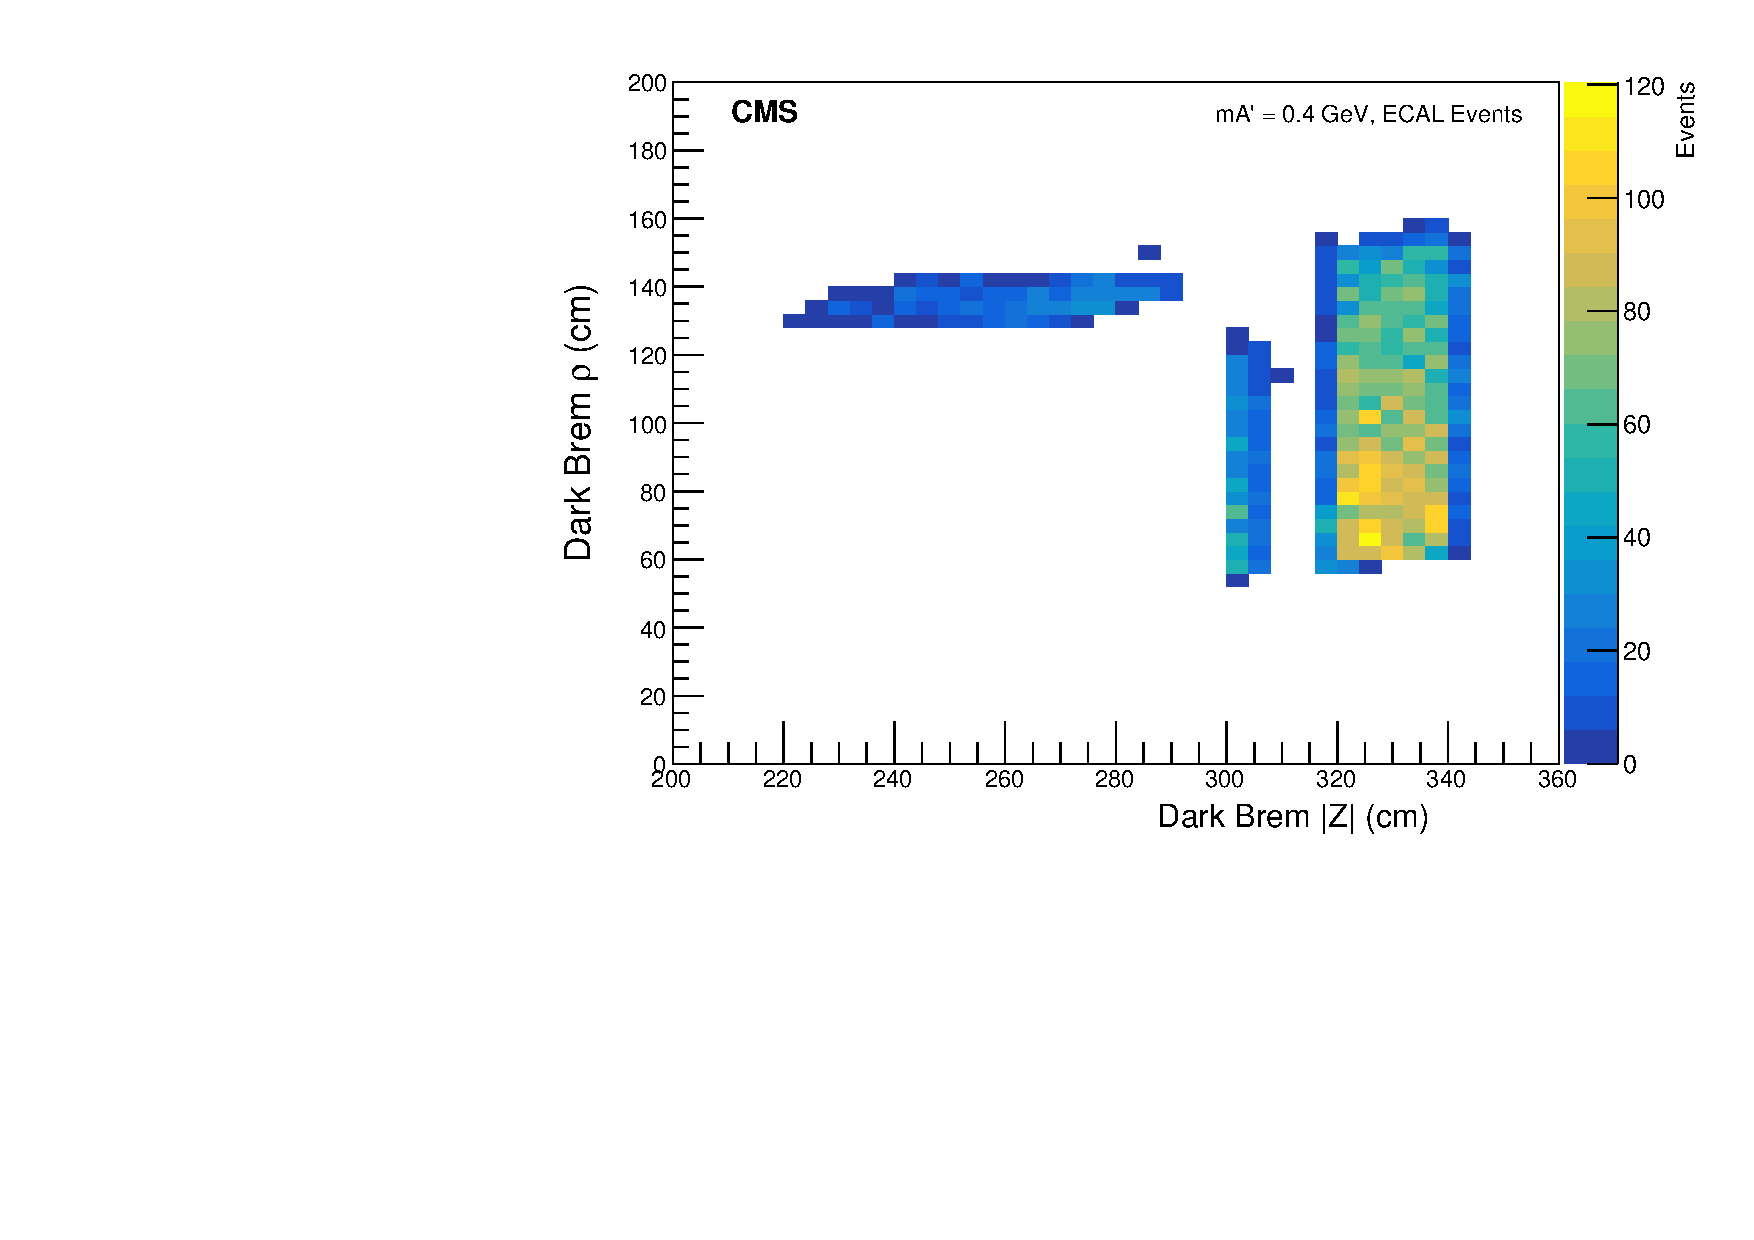
\includegraphics[width=0.9\textwidth]{figures/ECALbrems.pdf}
	\centering
	\caption{The locations of simulated \dbrem events within the CMS ECAL endcap}
	\label{fig:EEbrems}
\end{figure}

\begin{figure}[!htbp]
    \centering
    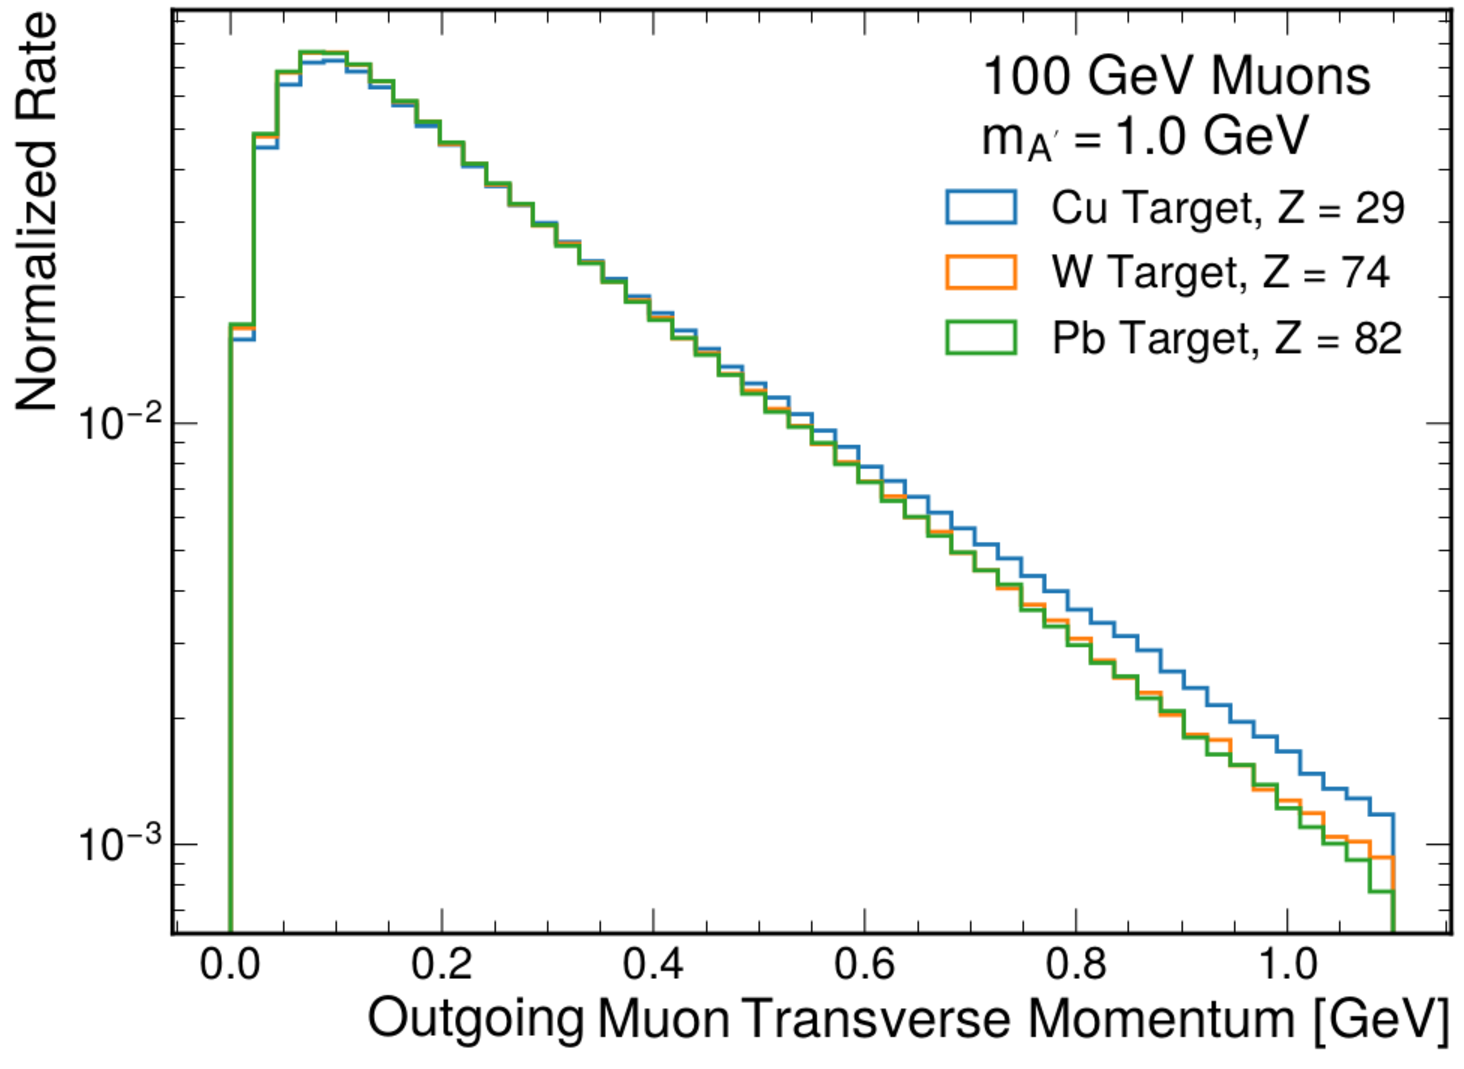
\includegraphics[width=0.45\textwidth]{figures/muon_material_comp_pt.pdf}
    \hspace{0.01\textwidth}
    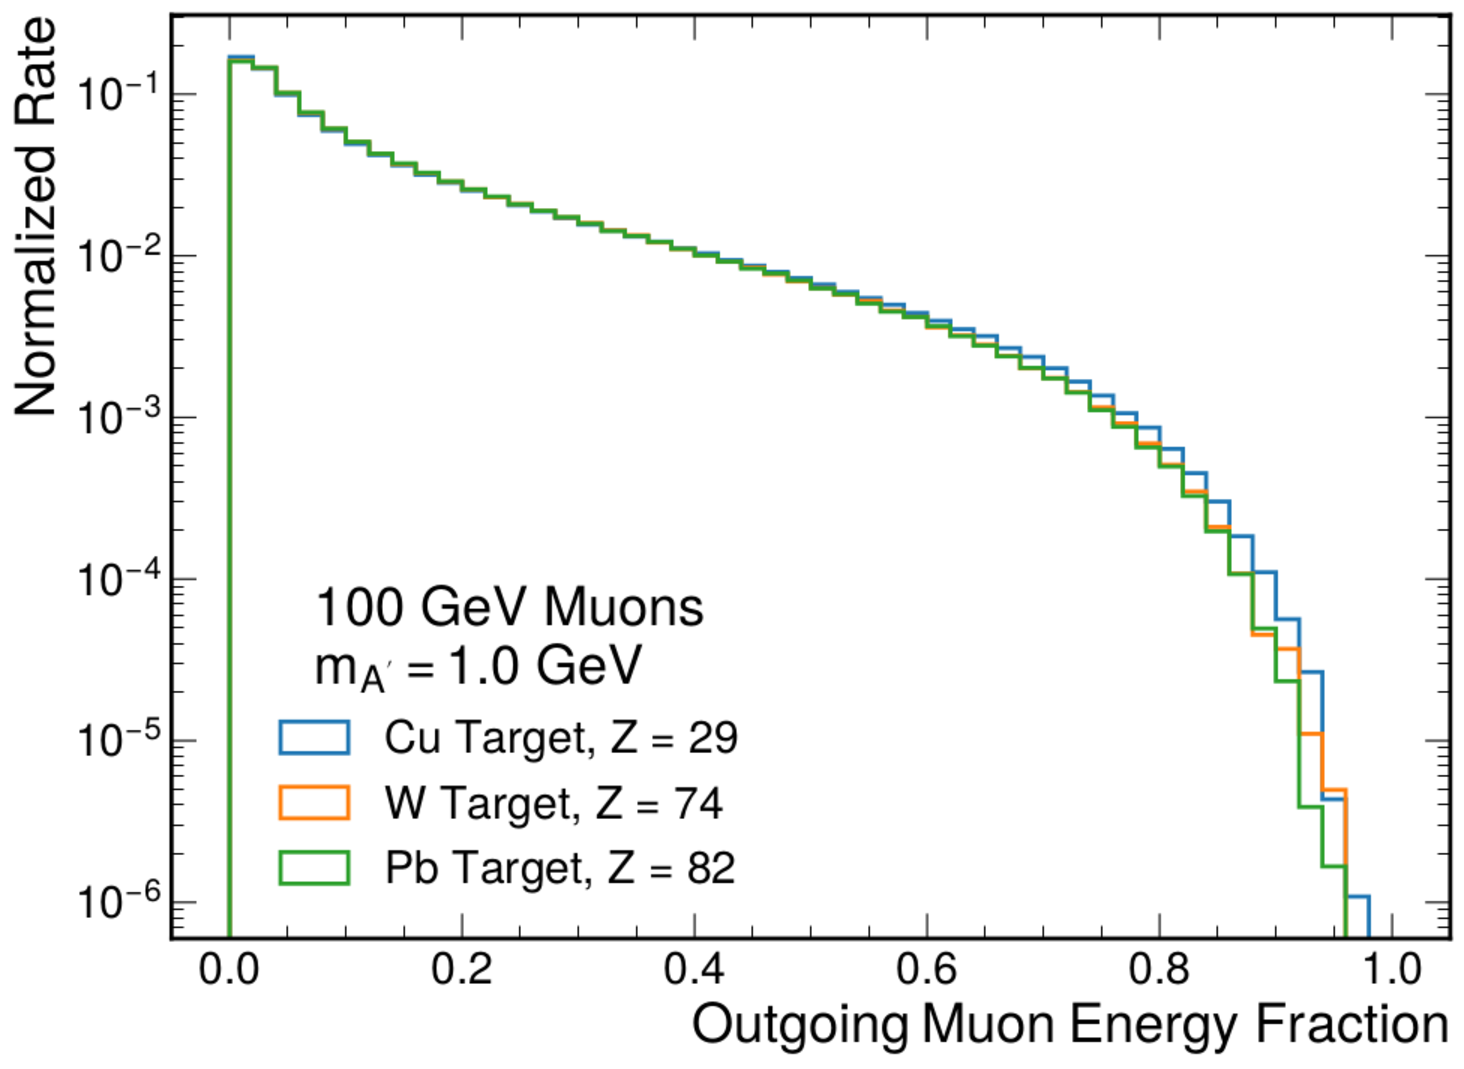
\includegraphics[width=0.45\textwidth]{figures/muon_material_comp_efrac.pdf}
    \caption[
        Material dependence of \dbrem kinematics.
    ]{
        The outgoing muon transverse momentum (left) and energy fraction (right) for muons incident on copper, lead, and tungsten. While materials close in Z have smaller relative shifts, the overall distributions are similar even with large changes in material. 
    }
    \label{fig:dbrem_material}
\end{figure}

\begin{table}[h]
    \centering
    \spacerows{1.2}
    \begin{center}
        \begin{tabular}{@{}l rr@{}}
            \toprule
            Material & 0.2 GeV & 1.5 GeV\\
            \midrule
            Copper&0.69&0.67\\
            Zinc&0.29&0.29\\
            Iron&0.02&0.03\\
            Chromium&0.004&0.01\\
            Carbon&0.002&0.003\\
            Nickel&0.001&0.005\\
            Hydrogen&0.001&0.0004\\
            Manganese&0.0004&0.0001\\
            Oxygen&0.0001&1.6$*10^{-5}$\\
            Nitrogen&3$*10^{-6}$&0\\
            \bottomrule
        \end{tabular}
        \caption{
            The fraction of \dbrem events initiated by detector material.
        }
        \label{table:dbrem_material}
    \end{center}
\end{table}
    
\section{Validation}
\label{sec:validation}

Comparing the recoil muon kinematics produced using this scaling procedure to a sample of \mg events at the target incident energy shows that this procedure does not significantly distort the distributions (\cref{fig:dbrem_validation}).
Moreover, these figures show that the scaling procedure more-closely resembles the ``true" \mg distribution the smaller the scaling distance is.

The outgoing muon angle is less well reconstructed using this procedure; however, the distributions stay within roughly 10\% of the \mg distributions for small scaling distances and scattering angles.
Large muon scattering angles are generally accompanied by very low outgoing energies, producing strongly signal-like events regardless of the outgoing angle. 
This procedure \emph{does not} reconstruct the sign of the outgoing muon's z-momentum, so it is always chosen to be positive. 
Due to the low rate of large scatters and the low outgoing muon energy of these events, the deviations seen above scattering angles of \SI{0.5}{\radian} do not significantly impact the signal efficiency.

\begin{figure}[!htbp]
    \centering
    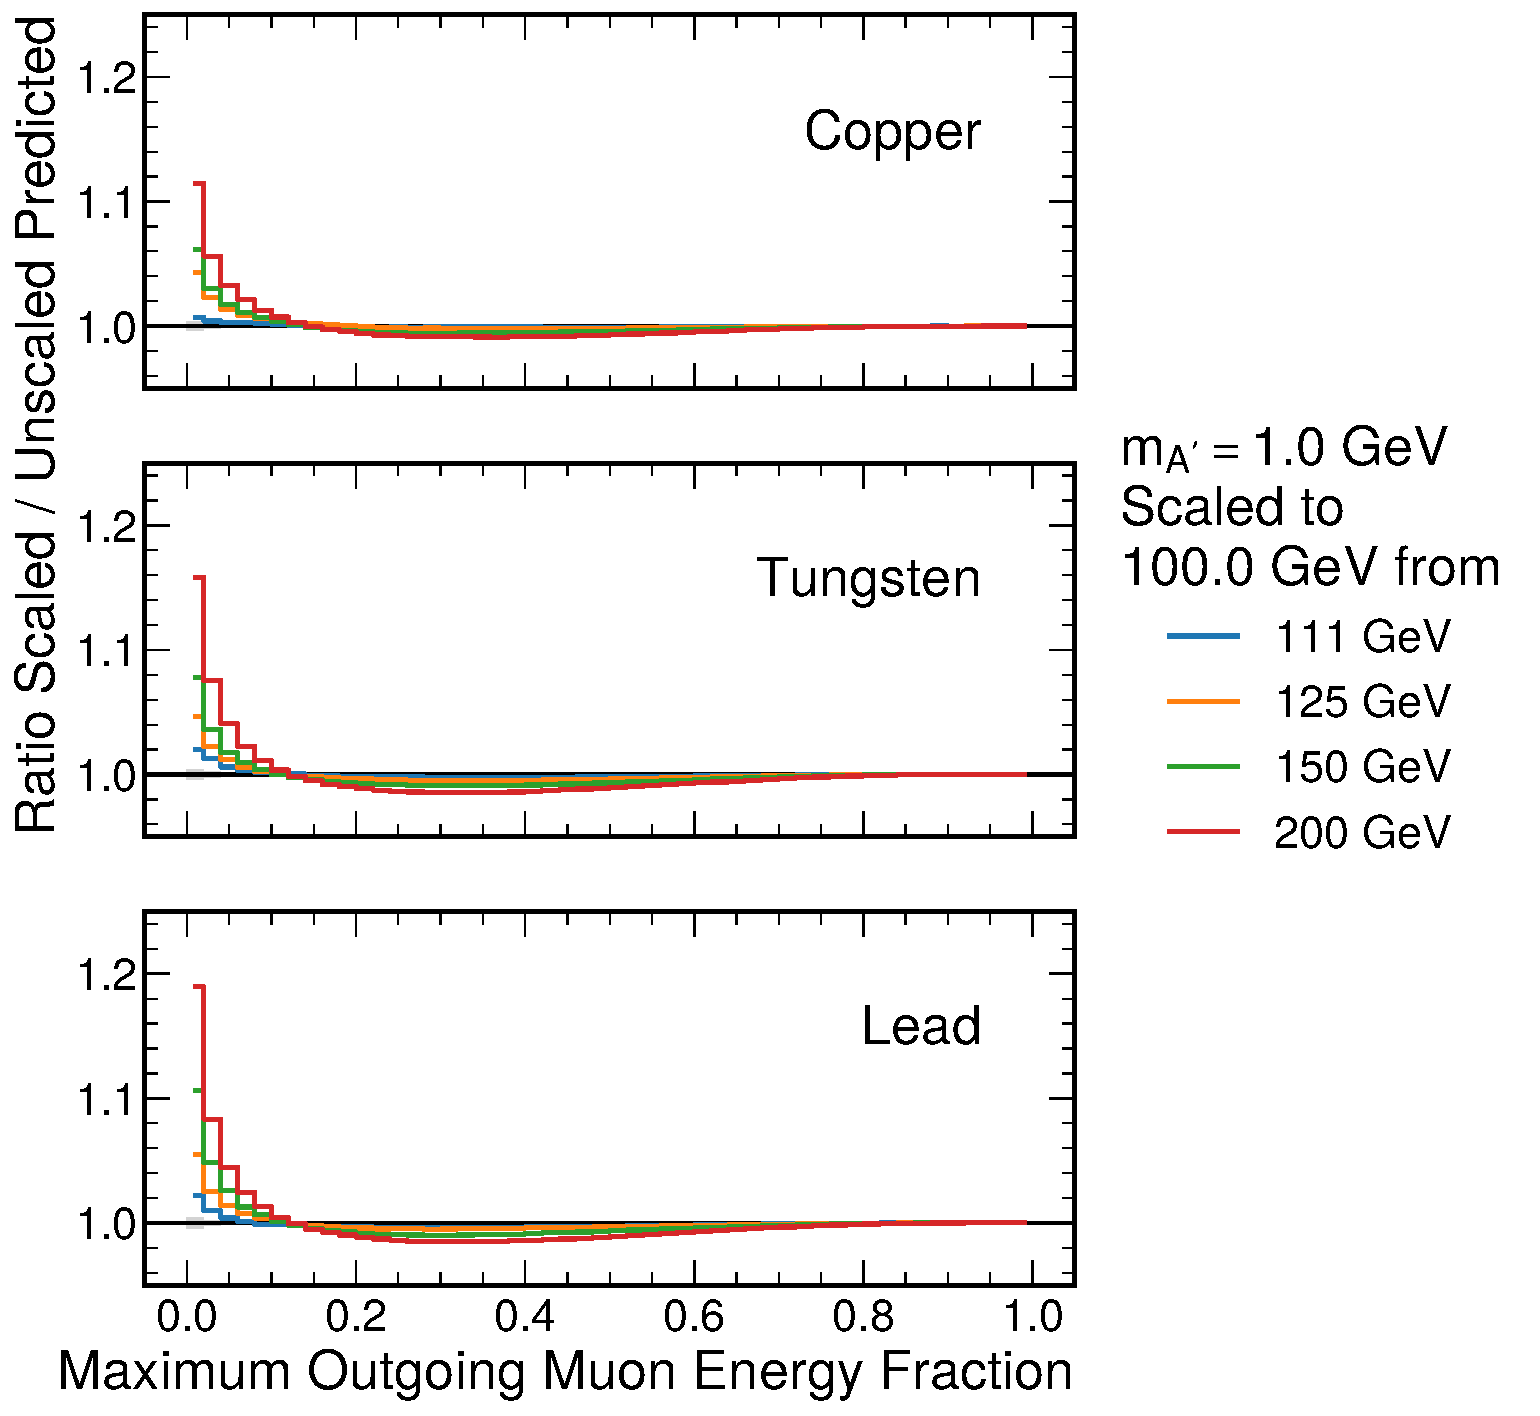
\includegraphics[width=0.45\textwidth]{figures/muon_efrac_cumulative_ratio.pdf}
    \hspace{0.01\textwidth}
    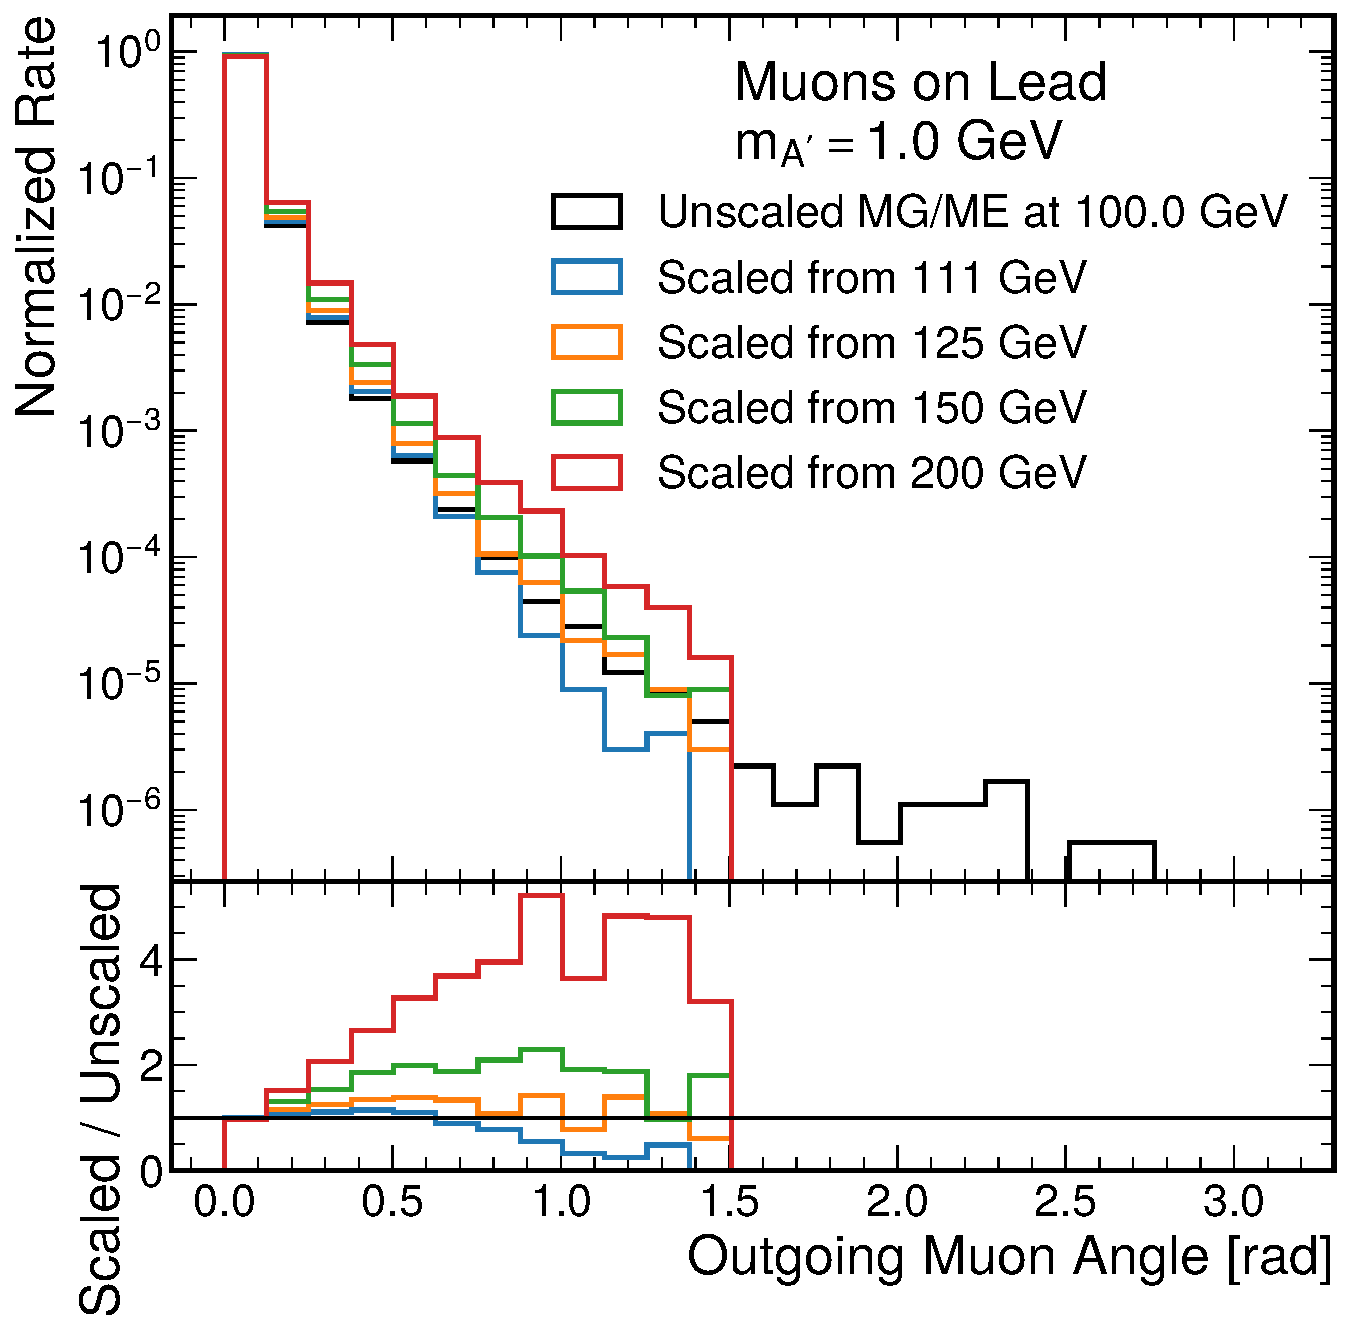
\includegraphics[width=0.45\textwidth]{figures/muon_lead_ang.pdf}
    \caption[
        Validation of simulated \dbrem kinematics.
    ]{
        The outgoing muon energy fraction for various scaling distances in copper, lead, and tungsten (left) and the muon deflection angle (right) for muons incident on lead.
    }
    \label{fig:dbrem_validation}
\end{figure}

\section{Fixed Target Luminosity}
\label{sec:fixedLumi}
When searching for a secondary interaction between a selected track and material in the detector, the relevant luminosity for the expected interaction rate is not the luminosity of the colliding beams but instead the 'fixed-target' luminosity of the probe muons passing through the detector.
Nominally, fixed target luminosity can be found from the product of the material density, the length traversed by the incident particles, and the total particle flux through the detector.
This first-principles luminosity could then be combined with the known \dbrem cross section to convert the observed event rate to a limit on $\epsilon$, but there are several complications that make such a calculation unfeasable.

As the total cross section is dependent on the kinetic energy of the probe, it depends both on the energy distributions of the selected probe tracks and any energy loss from ionization or scattering as it traverses HCAL.
Additionally, the non-uniform geometry of HCAL can cause significant variations in the active material depth for muons with different positions and energies. 
A full estimate of the fixed target luminosity from first principles would need to calculate the amount of material along any arbitrary trajectory in HE, then combine this with the observed distribution of all selected probe trajectories and energies to find the average product of luminosity and cross section to relate the mixing parameter to the produced event rate.

To avoid the complications of calculating it directly, the fixed target luminosity is instead determined from the signal simulation.
The probability for any given muon to have a \dbrem interaction is the product of the cross section and luminosity for its particular trajectory, as long as the interaction rate is small.
Large cross sections lead to non-physical events with multiple \dbrem interactions, or concentrations of \dbrem events near the front of the detector due to the reduction in cross section in deeper parts of the detector from energy loss to earlier \dbrem. 
The fraction of events with a \dbrem interaction is shown in \Cref{eq:mcrate}, where $n_{mc}$ is the interaction rate and $\langle \sigma_0 l \rangle$ is the average product of the fixed target luminosity $l$ and the cross section with epsilon set to one, $\sigma_0$.  

By generating large numbers of events with muons incident on the endcap with bias factors small enough to ensure this linearity in interaction rate, the observed rate within the simulation can be used to find the average product of cross section and luminosity without needing to separate the two terms.
As long as the simulated muons have the same kinematics as those in data, the rate of signal events in data (\Cref{eq:datarate}, where $n_{data}$ is the observed event rate) can be divided by this product from simulation to relate the number of signal events observed to the value of the mixing parameter required to produce that rate, creating a conversion from limits set in the rate of signal events per incident muon to limits on the mixing parameter itself (\Cref{eq:fixedLumi}).

\begin{equation}
	\label{eq:mcrate}
	n_{mc} = \epsilon_{mc}^2 \langle \sigma_0 l \rangle
\end{equation}

\begin{equation}
	\label{eq:datarate}
	\epsilon^2 = frac{n_{data}}{\langle \sigma_0 l\rangle}

\begin{equation}
	\label{eq:fixedLumi}
	\epsilon^2 = \frac{n_{data}\epsilon_{mc}^2}{n_{mc}}  
\end{equation}

Due to the use of signal events per selection muon, the final limits on $\epsilon$ have no direct dependency on the collision luminosity and so avoid its associated luminosity uncertainty, but instead have uncertainty related to the accuracy of the modeling of the detector.
While the CMS detector is calibrated to accurately simulate its response to energetic particles, the simulation may have small variations in the simulated geometry that are resolved through energy response calibration when they are really produced by material simulation differences.
This systematic uncertainty is estimated by assuming that it may result in at most one more or one less absorber layer along the trajectory of any given muon, producing overall $\pm$5$\%$ and $\pm$5$\%$ systematic uncertainties within the HCAL and ECAL, respectively.

\begin{figure}[h]
	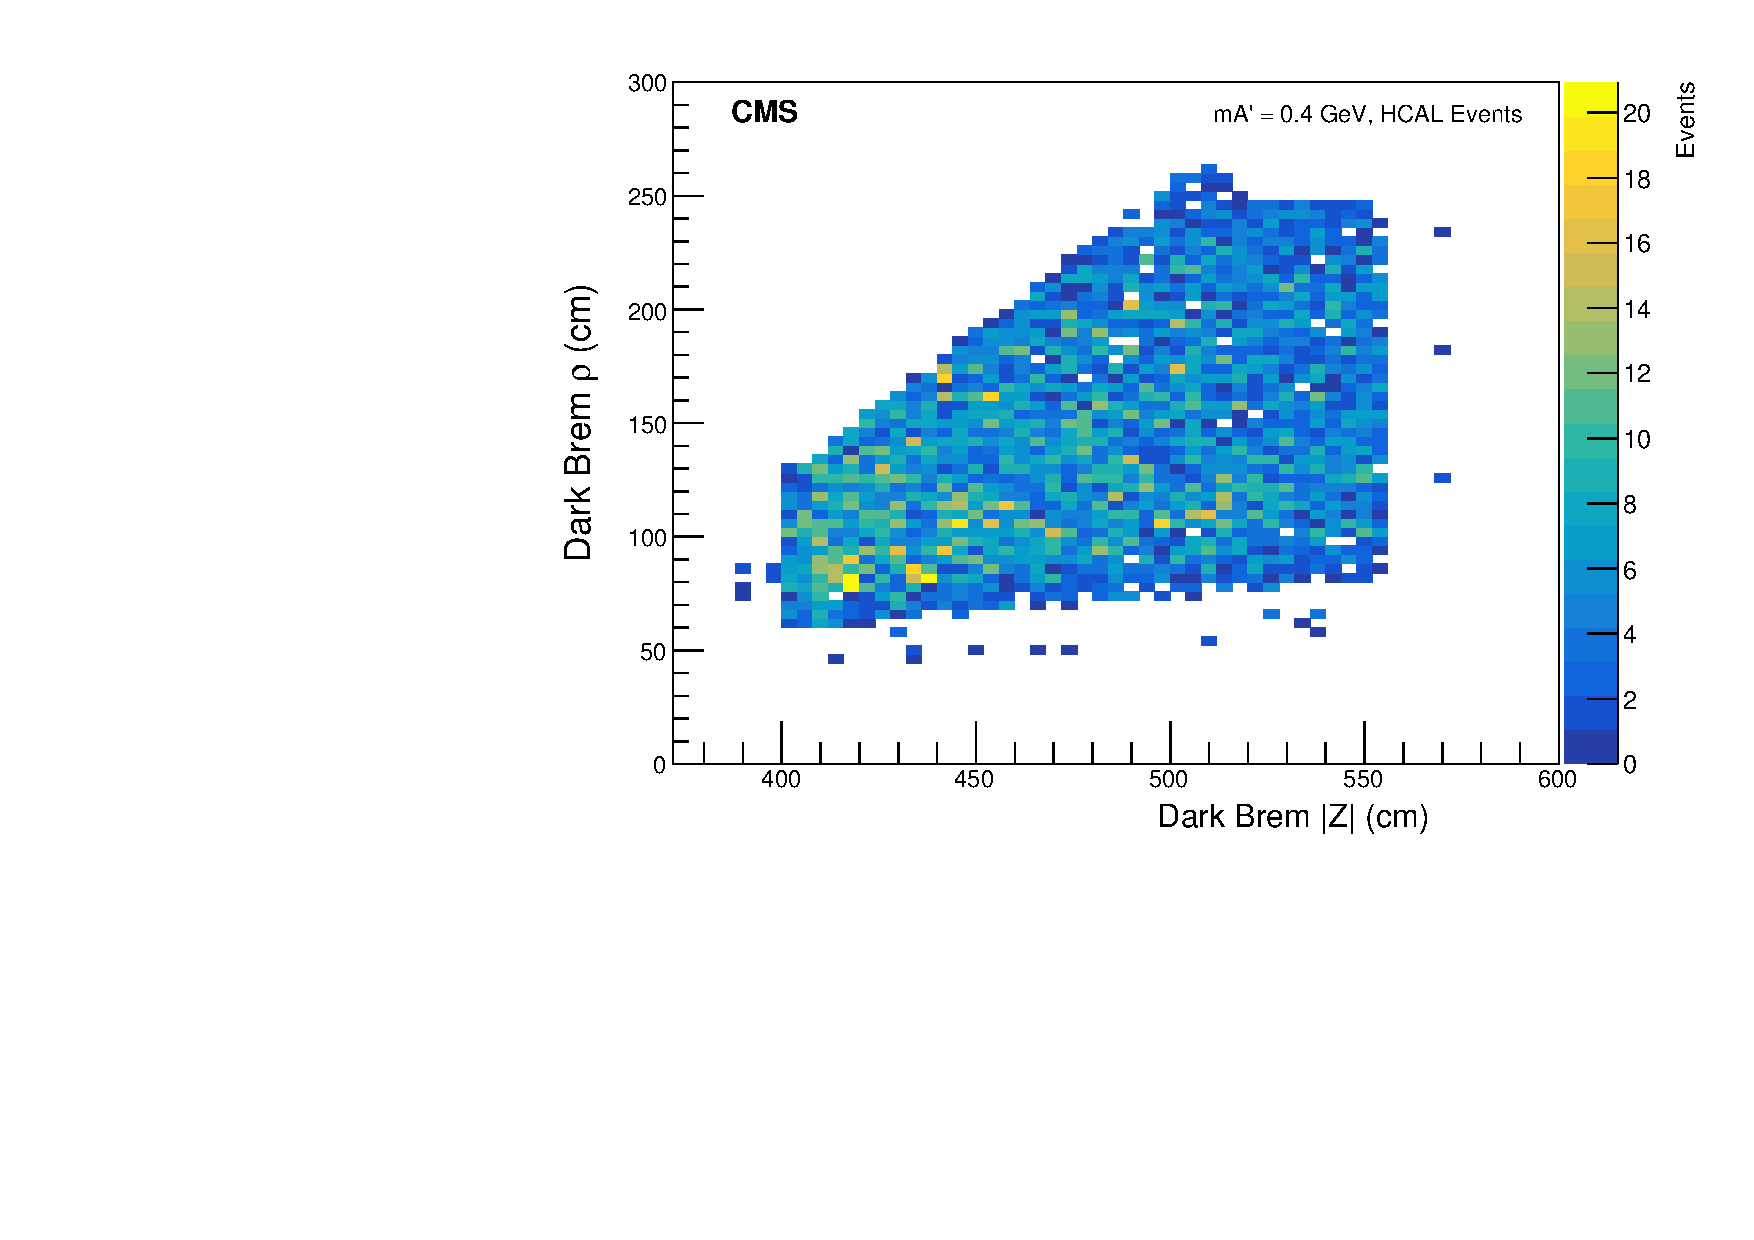
\includegraphics[width=0.9\textwidth]{figures/HCALbrems.png}
	\centering
	\caption{The locations of simulated \dbrem events within the CMS HCAL endcap}
	\label{fig:HEbrems}
\end{figure}

\begin{figure}[h]
	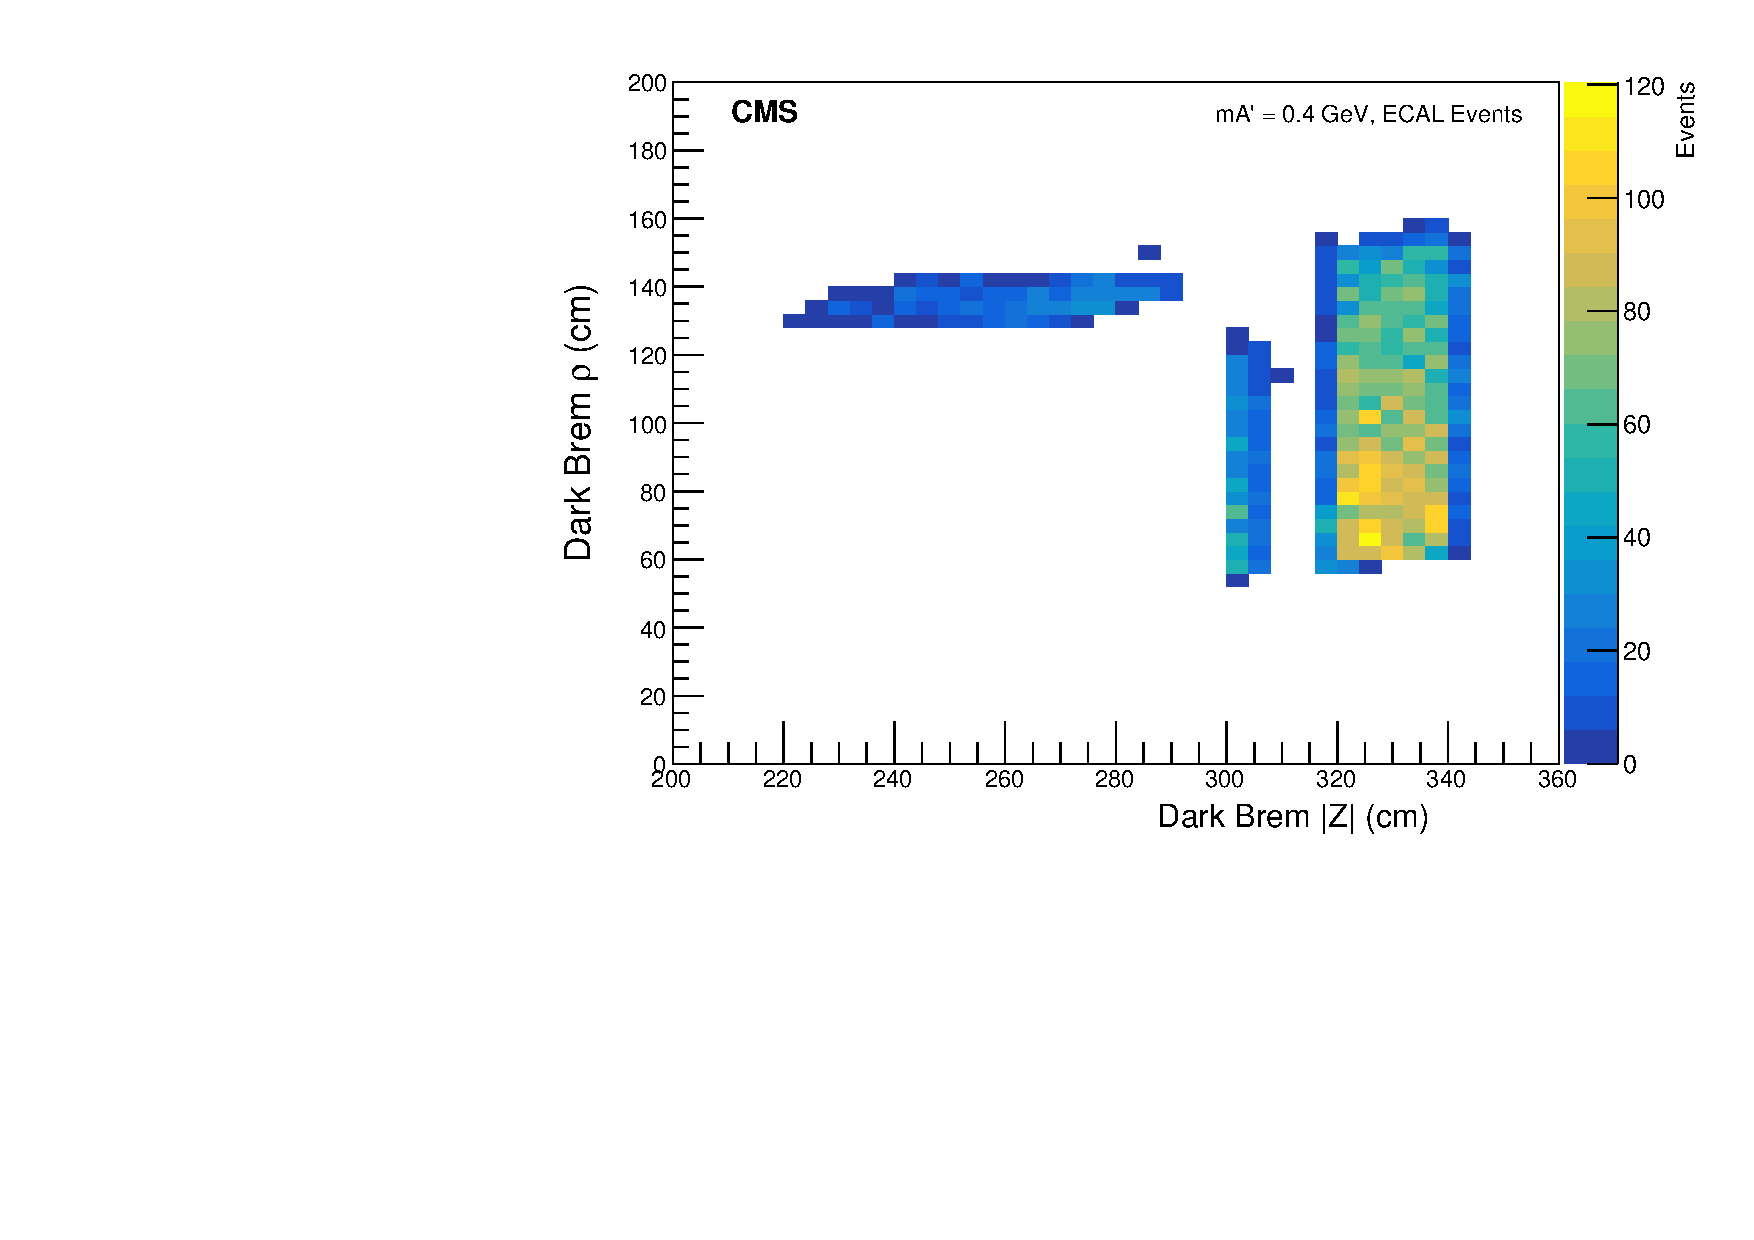
\includegraphics[width=0.9\textwidth]{figures/ECALbrems.png}
	\centering
	\caption{The locations of simulated \dbrem events within the CMS ECAL endcap}
	\label{fig:EEbrems}
\end{figure}


